\chapter{Answering questions with astronomical images}

Last week, you queued up some images to be taken by the robotic telescope and learned how telescopes work to create images. This week, you'll learn how we record these images, and you'll learn one way to analyze those images to create knowledge about the distance between stars.

\section{Learning goals}

\begin{itemize}
	\item Answer questions by analyzing data that you took yourself.
	
	\item Experience and analyze the light gathering and angular resolution benefits of telescopes.
	
	\item Use pixel scale and length measurements to determine the angular separation of objects in a digital image.
	
	\item Gain insight of and appreciation for the scale of astronomical distances.
\end{itemize}



\section{How big is your face?}

This is a simple question, so that you can learn some astronomical concepts and tools while answering it and still keeping the subject matter intuitive.

\subsection{Background: reflecting telescopes and CCDs}

The primary utility of a telescope is its ability to gather light, thereby enabling visualization and analysis of the faint astronomical objects we are trying to observe. This requires focusing light incident on a large surface area. We will be using a \textbf{reflecting} telescope, which means that light rays from observation targets are focused into an eyepiece or onto a detector with reflecting mirrors. This is in contrast to refracting telescopes, which use refracting lenses to focus light rays. Figure~\ref{sot:fig:schmidt} shows schematically how this kind of telescope works. 

\begin{figure}
	\centering
	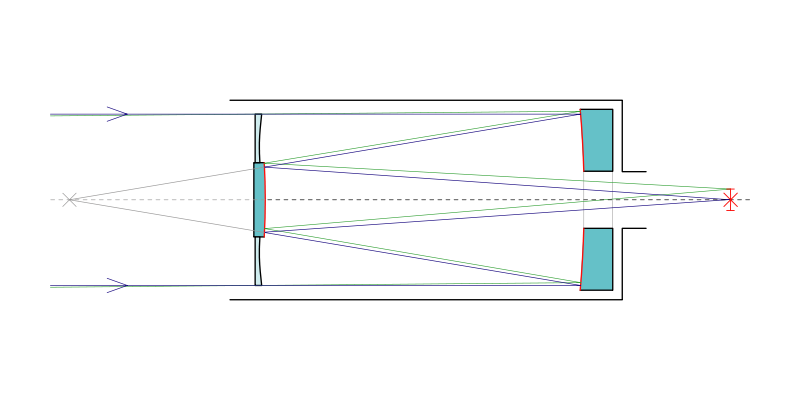
\includegraphics[scale = 0.5]{small-optical-telescopes/Schmidt-Cassegrain-Telescope.png}
	\caption{Schematic for a reflecting telescope of a Schmidt-Cassegrain design. 
		Light rays from astronomical objects enter the telescope in parallel because their source is effectively at infinity. They are then reflected by a parabolic primary mirror onto a secondary mirror that again reflects the light to a focus. An eyepiece or a camera is placed at the focal plane of the resulting image. Image source: \url{https://en.wikipedia.org/wiki/Cassegrain\_reflector\#/media/File:Schmidt-Cassegrain-Telescope.svg}}\label{sot:fig:schmidt}
\end{figure}

To take images in this lab, and to observe astronomical objects using the SEO, we make use of a \textbf{Charge Coupled Device (CCD)}. CCDs are the standard detectors for taking astronomical images at wavelengths blueward of approximately 1 micron. Think of the CCD we are using as a
very advanced low-noise digital detector, not wholly dissimilar from the digital detector in your
smartphone. Every time a photon within a certain energy range hits the detector, an electron is knocked off of the incident pixel, charging that pixel's capacitor. Thus, for each pixel, more photons $\implies$ more electrons $\implies$ more charge, and the charge can be read off into a digital signal that is then processed as an image. 

The main thing to note is that the CCD material is not sensitive to all wavelengths of light uniformly. Photons of certain energies are more likely to excite electrons in the detector and thus contribute to the output image. Consequently, the observed image intensity will be weighted by the response function of the detector.

\subsection{Telescope Set Up, Preliminary ``Observations"}\label{ai:sec:setup}

The telescope and camera assembly is an expensive and relatively fragile piece of hardware, so
move carefully when interacting with the system. We have only two setups, so the class will be split into two groups for using the classroom telescope.

First we will be observing an object at the opposite end of the lab room with the lights turned off. During this exercise we will 1) check that the telescope is focused (which should already be the case), 2) gain practice positioning the telescope and targets, and 3) demonstrate the light gathering and angular resolution capabilities of the telescope with a physical object for which you have an direct sense of scale. \textbf{NOTE: For safety purposes, do not walk around the
	lab while the lights are off; instead, turn the lights off only as needed to gather data
	or make observations, and when the lights are off, don’t move about significantly.}

\begin{steps}
	\item The telescope should already be set up, with the camera on and cooled, and be approximately
	in focus and pointed at the target at the other end of the lab bench. If not, your TA will
	work with you to get the setup roughly correct.
	
	\item Your first task will be to tweak the centering of the image target. This doesn’t have to be
	perfect, but you should be able to see the mm scale marks. The telescope can be moved in elevation (up-down). The fine control of elevation is achieved using a knob on the mount - your TA will show you details. To shift the image left or right, move the target instead.
	
	\item Next we want to precisely focus the telescope. Do this with most of the lights off --- otherwise
	the image has too much light. Use the 4th filter of the five available; this can be selected
	from the ‘Filter’ menu. Then, use the \textbf{Focus} task from the camera control system toolbar,
	and take images of a few seconds (at most). If the image is completely dark, and the peak intensity number in the focus box is reading around 65000, then the CCD is saturated, and the light in the room should be reduced, or the exposure time shortened.
	
	\item Start the focus sequence - the camera will just
	take and display images repeatedly, of the exposure duration you specified. Now, adjust
	the focus knob (on the back of the telescope, off center) until you achieve an optimal focus.
	Note that you can (and should) zoom the magnification of the image so you can see the
	imaging target in detail. Do this by adjusting the magnification, and adjusting the image
	x,y centering so you’re looking at an appropriate zoomed location in the image. Note that
	you’ll need to not be touching the telescope or mount to get a sharp image, so you’ll
	have to adjust, then move away, wait, and repeat. Your classmates walking around the lab
	will cause image shake that will make focusing difficult, so enforce a still classroom while
	you do this.
	
	\item Time to demonstrate one helpful aspect of telescopes by taking an image in the dark. Once the telescope is focused to the sharpest possible images, turn off the lights and acquire an image using the
	\textbf{Grab} button on the toolbar. An exposure time of 40--60 seconds is usually good with all of
	the lab lights off and the blinds closed.
	
	\item Save this image in ‘fits’ format; the ‘ds9’ tool available on all of the lab
	computers can be used to examine the image in detail. You can use the university supported
	’Box’ system to share data with your lab classmates. See \url{uchicago.account.box.com/login}
	for details.
	
	\item With the lights back on, gather around the target on the lab bench and then
	turn the light off again. Observe the target. Can you see it? Can you see the details? Does
	it matter how close you are (Rubric Row B5)?
	
	\item Compute and report the ratio of the light gathering power of
	the telescope relative to your eye, and comment on how that relates to what you do (or do
	not) observe by eye compared to the telescope (Rubric Row B9).
	
	\item In the acquired and saved image you can see a mm scale, which correponds to some number
	of pixels. Compute and report the ‘plate scale’ in mm/pixel. Given the distance between the
	telescope and the target, what is the angular plate scale in arcseconds/pixel?
	
	To find this, note that for an arc (segment) of a circle, the length of that arc $s$ is related to the radius of circle $r$, and the angle (in radians) subtended by that arc $\theta$ by
	\begin{equation}
	s = r \theta
	\end{equation}
	
	\item What do you
	think is the smallest feature (in arcsec) that you could resolve using this setup? Would we
	expect to see images of stars that sharp if we turned the telescope and camera skyward?
	Also, what is the field of view (arcseconds $\times$
	arcseconds) of this camera+telescope setup? Finally, observe the target from the vantage
	point of the telescope by eye. What detail can you see? How does that compare to what
	you can see with the telescope?
	
	\item Now take an image of part of one of your groupmates with the telescope. Centering on their eye can make for a fun picture. Use the pixel scale that you determined, along with that image, to find the angular separation (or ``angular distance'') between two points in the image --- for example, what is the angle subtended by their eye? Use the distance from the telescope to the person to also determine the distance between those two points, for example in millimeters. Estimate your uncertainty and compare this measurement to a direct one (by holding up a ruler, for example.)
\end{steps}

\section{How far apart are these stars?}

Now that you have experience measuring distances for objects you can directly measure, you'll try your hand at measuring distant objects that none of us can measure directly --- other stars in your image from SEO! The goal here is to pick two stars in your image and find the angular separation between them, as well as physical distance. To get the physical distance, you'll need to know their distances from Earth. To get that, you'll need to match up those stars in your image to known stars. You can use Stellarium for this, a free virtual observatory app. Then you can select those stars in the app and easily find information about them.

Note that since we are using a real robotic telescope, many things can go wrong that may result in you not having an image that you've taken. There could have been cloudy nights all week, or smoke from wildfires, or planned power outages to protect from wildfires, or part of the observatory could have broken down. We have archival images in the case that your images are not taken, so that you can still complete the lab.

\begin{steps}
	\item Log into \url{queue.stoneedgeobservatory.com}, find your completed observation, and click ``go to image''. If you don't have a completed observation, find a classmate's or TA's image URL to visit to get an image to work with. If the image that appears is very fuzzy or has no stars in it, choose a different option from the ``Pipe Step'' drop-down menu.
	
	\item Select the link ``Download Selected FITS File'' to do so. Open it in DS9.
	
	\item Also open Stellarium on a computer. It is a free open source virtual observatory, so you can install it on your computer if you'd like. Use Stellarium to find your target. Zoom in by selecting the rectangle icon third from the right in the upper-right-hand corner. This simulates a field of view that is similar to our telescope.
	
	\item Use the Stellarium view to identify two stars from your image. The two pictures might be rotated relative to each other.
	
	\item For those two stars, use DS9 to measure the angular separation (angular distance) between them. \textbf{Record this and your uncertainty for it.}
	
	\item In Stellarium, select each of the two stars in turn and record their equatorial coordinates (RA/Dec J2000.0). Calculate the angular separation using a web form, for example \url{http://hea.iki.rssi.ru/AZT22/ENG/cgi-bin/c_dist.htm}.
	
	\item Use the $t'$ statistic (see Appendix\ \ref{unc:sec:comparing}) to compare these two values of angular separation.
	
	\item To find the physical distance between them, use the distances from Earth as given in Stellarium, along with the angular separation and some geometry.
	
	\item How long does it take light to travel from one of those stars to the other?
\end{steps}

\section{But wait! Next set of observations with SEO}

In the next lab, we will be exploring the use of color in astronomical images. The CCD image sensor is monochrome. That is, it has a relatively flat sensitivity to different wavelengths in the visible spectrum. To gain information about color, or the relative contributions of different wavelengths, you'll use filters that can be placed in front of the sensor. So for next week, \textbf{queue another observation or several} (no more than 1 per student per week). Choose the same target from last week. Select the r, g, and b filters (red, green, and blue, respectively), and leave the "dark" checked as well. For the exposure time, you can adjust it if you think the image was over- or under-exposed, but be careful --- the color filters cut down the intensity of light, even in the color that it transmits the most, by at least a factor of two.

\section{Report checklist and grading}

Each item below is worth 10 points, and there is an additional 10 points for attendance and participation. See Appendix\ \ref{cha:lab-report-format} for guidance on writing the report and formatting tables and graphs.

\begin{itemize}
	
	\item 
	
\end{itemize}